\documentclass[10pt]{article}

% Lines beginning with the percent sign are comments
% This file has been commented to help you understand more about LaTeX

% DO NOT EDIT THE LINES BETWEEN THE TWO LONG HORIZONTAL LINES

%---------------------------------------------------------------------------------------------------------

% Packages add extra functionality.
\usepackage{
	times,
	graphicx,
	epstopdf,
	fancyhdr,
	amsfonts,
	amsthm,
	amsmath,
	algorithm,
	algorithmic,
	xspace,
	hyperref}
\usepackage[left=1in,top=1in,right=1in,bottom=1in]{geometry}
\usepackage{sect sty}	%For centering section headings
\usepackage{enumerate}	%Allows more labeling options for enumerate environments 
\usepackage{epsfig}
\usepackage[space]{grffile}
\usepackage{booktabs}
\usepackage{amsmath}
\usepackage{qtree}
\usepackage[super]{nth}

% This will set LaTeX to look for figures in the same directory as the .tex file
\graphicspath{.} % The dot means current directory.

\pagestyle{fancy}

\lhead{\YOURID}
\chead{\MyLang: Language Specification}
\rhead{\today}
\lfoot{CSCI 334: Principles of Programming Languages}
\cfoot{\thepage}
\rfoot{Spring 2020}

% Some commands for changing header and footer format
\renewcommand{\headrulewidth}{0.4pt}
\renewcommand{\headwidth}{\textwidth}
\renewcommand{\footrulewidth}{0.4pt}

% These let you use common environments
\newtheorem{claim}{Claim}
\newtheorem{definition}{Definition}
\newtheorem{theorem}{Theorem}
\newtheorem{lemma}{Lemma}
\newtheorem{observation}{Observation}
\newtheorem{question}{Question}

\setlength{\parindent}{0cm}
%---------------------------------------------------------------------------------------------------------

% DON'T CHANGE ANYTHING ABOVE HERE
\begin{document}

\newcommand{\YOURID}{Jared Berger}	% Replace "Your Name Here" with your name
\newcommand{\MyLang}{Arpeggify}	% Replace MyLang with your language name #
\newcommand{\ProblemHeader}	% Don't change this!



\vspace{\baselineskip}	% Add some vertical space

% Refer to the lab handouts to determine what should go in each of these sections.  Each lab is additive.  So lab 8 should include everything you wrote in lab 7.  Lab 9 should include everything you wrote in lab 8, etc.

\section{Introduction}

My programming language (tentatively named Arpeggify) solves the problem of automatically arpeggiating chord progressions (ie. successively playing the notes in a piece of music's chords). Having this language first can assist musicians with composition and allows them to experiment with and immediately hear different chord progressions. Rather than having to write out sheet music, potential composers could specify chord names and immediately hear what they would sound like together, without the need for any instruments. Second, this language could help musicians practice. After encoding a piece of music as a program, musicians could listen to and observe the piece's harmony and potentially practice along to it.

This problem needs its own programming language because there are infinitely many pieces of music, each defined by a grammar. The harmony of a piece of music can be broken down into sections, phrases, individual chords, and the individual notes within those chords, and I think this structure might lend itself to being interpreted as a programming language rather than simply an input to a single program. Solving this problem with a programming language allows programmers to follow a set of rules to generate and infinite number of programs, all while exploring the idea of a piece of music being used as a computer program.

\section{Design Principles}
The guiding principles are the parallels between music compositions and programs. I'm thinking particularly about lead sheets for jazz tunes, which provide visual representations of the structures of tunes. Encoded in this sheet music is information about which chords go where, which types of chords are played, in addition to a feel for the overall structure of the piece. Many jazz compositions are in the form of an "A" section repeated twice, followed by a "B" section then by an "A" section again, and I'm interested in finding a way to capture these common sections and relationships between them in my language. Further, in my implementation or arpeggiation, I am aiming to make the language be easily extendable and for more chord types and features to easily be added. I've created a general interpretation for arpeggiating chords, which involves representing each note as a numeric value and then calculating the notes in a chord and their corresponding frequencies using formulas. This keeps large parts of my code generic, and allows for new types of chords to be defined and to work right away.

\section{Example Programs}
\textbf{**For now, a sample program is a command line argument. 
Here is an example that works in my minimally working language:}
\begin{verbatim}
    dotnet run "(E-7,A7,D-7,G7)(4,4,4,4)||" output.wav
\end{verbatim}

Here are more advanced examples that will eventually work:

1) A simple 3-6-2-5 chord progression in C
\begin{verbatim}
    chords c = (E-7, A7, D-7, G7)
    rhythm r = (4 -> all)
    phrase p = (c,r)
    tune t = p:||
\end{verbatim}

2) A 12-bar "C" blues
\begin{verbatim}
// chords found in a, b, and c sections
chords aChords = (C7, C7, C7, C7)
chords bChords = (F7, F7, C7, C7)
chords cChords = (G7, F7, C7, C7) 

rhythm rA,rB,rC = (4 -> all)

// combine chords and chord lengths to form phrases
phrase A = (aChords, rA)
phrase B = (bChords, rB)
phrase C = (cChords, rC)

// combines phrases into a tune
tune Blues = A + B + C:||
\end{verbatim}

3) The jazz standard "I've Never Been in Love Before"
\begin{verbatim}
    // chords found in a, b, and c sections
    aChords = (Bb6, G-7, C-7, F7, BbMa7, Eb7, D-7, G7, C-7, F7)
    bChords = (EbMa7, C-7, F7, BbMa7, A-7, D7, G-7, 
                C7, Eb7, DMa7, C-7, B7)
    
    // chords in first and second endings of a section
    e1Chords = (BbMa7, C-7, F7)
    e2Chords = (BbMa7, F-7, Bb7)
    
    rhythm rA = (2,2,2,2,2,2,4,4)
    rhythm rB = (4,2,2,4,2,2,4,2,2,4,2,2)
    rhythm re1, re2 = (4,2,2)
    
    // combine chords and rhythms into phrases
    phrase A = (aChords, rA)
    phrase B = (bChords, rB)
    phrase e1 = (e1Chords, re1)
    phrase e2 = (e1Chords, re2)
    
    // combine phrases to form a tune
    tune neverBeen = A + e1 + A + e2 + B + A + e1 ||
\end{verbatim}

\section{Language Concepts}

To write Arpeggify programs a user needs to understand nomenclature for jazz chords and an understanding of how chords can be combined to build phrases, and, in turn, tunes. A programmer would need knowledge of note names and common chord extensions. Experimentation would of course be encouraged, but the they would also need a basic understanding of harmony in order for the program output to sound good.

\section{Syntax}
For now, my language only works with a program entered as a command-line argument. My minimal formal grammar is:

\begin{verbatim}
    <tune>       ::= <phrase>
    <phrase>     ::= <chord><rhythm>
                  | <chord><rhythm><phrase>
    <rhythm>     ::= x in (1,2,3,4...)              
    <chord>      ::= <root><extension>
    <extension>  ::= <Major7><Minor7><Dom7>
    <root>       ::= <note>
                  | <accidental>
    <note>       ::= x in (A,B,C,D,E,F,G)
    <accidental> ::= <note><symbol>
    <symbol>     ::= #
                  | b
              
\end{verbatim}
The language is built of tunes which are created through combinations of phrases and repeats. I'm imagining that eventually programmers could use the "+" operator to combined phrases into a complete tune, followed by a symbol to indicate that the piece either ends or repeats. Phrases, then, are built out of rhythms and chords. Rhythms such as "2" or "4" represent the length of their corresponding chords. For example, a chord meant to be played for 2 beats would have a corresponding rhythm of a "2". Chords are made up of a root and an extension. A root is simply a note name like "E" and an extension indicates the type of chord (eg. major, minor, diminished). Chords are made by combining roots with extensions in the form of \verb{<root><extension>}

\section{Semantics}

\textbf{Minimal Semantics:}
\begin{table}[thb]
\centering
\begin{tabular}{|l|c|l|l|l|} \hline
\textbf{Syntax} & \textbf{Abstract Syntax} & \textbf{Type} & \textbf{Prec.} & \textbf{Meaning}\\ \hline
(E-7,A7,D-7,G7)(4,4,4,4) & Chord List * Rhythm List & Phrase & Left first & This is a phrase built of a list of \\ & & & & chords and a list of rhythms. Each chord \\ & & & & listed will be played for 4 beats. \\ \hline
E-7 & Root * Extension & Chord & N/A & This is a chord built out of a root and \\ & & & & extension. The root of the chord is E and \\ & & & & the other notes in the chord are G, B, \\ & & & &  and D, to complete the minor 7th chord. \\ \hline
Ab & Accidental of Root * Symbol & Root & N/A & This is a root built of a note and \\ & & & & a symbol. This is represented as the note 'A' \\ & & & &lowered by a half-step due the to presence\\ & & & & of the "b" symbol. \\ \hline
(E-7,A7,D-7,G7)(4,4,4,4)\|\| &  Phrase list * Ending & Tune & N/A & This is a complete tune, \\ & & & &built of a phrase list containing one phrase, \\ & & & &which contains four chords each played for 4 \\ & & & &beats each, and then an ending indicating \\ & & & &  that the tune is over.\\
\hline\end{tabular}
\end{table}

i. The primitive kinds of values are notes, rhythms, and symbols. Notes and symbols combine to form chords and extensions and these combine with rhythms to form phrases. From these primitives we can build an infinite number of phrases and tunes using our 12 possible roots (the 12 notes), a predefined set of extensions(types of chords), and rhythms within a specified range.

ii. The values are used to tell the computer which frequencies to generate and in which order an for what length. Within a tune or phrase, the structure of a chord tells the computer which nodes are to be synthesized, and the rhythm tells the computer how long each note should be played for. The values used in our programming language are converted into sounds which arpeggiate the desired chord progression. Operations combine primitives (like roots and extensions) into larger structures, yet the information in these primitives indicates which basic sounds are to be created.

iii. Our program is represented as an overall tune, composed of phrases, which are composed of chords and rhythms. 

This might look something like:

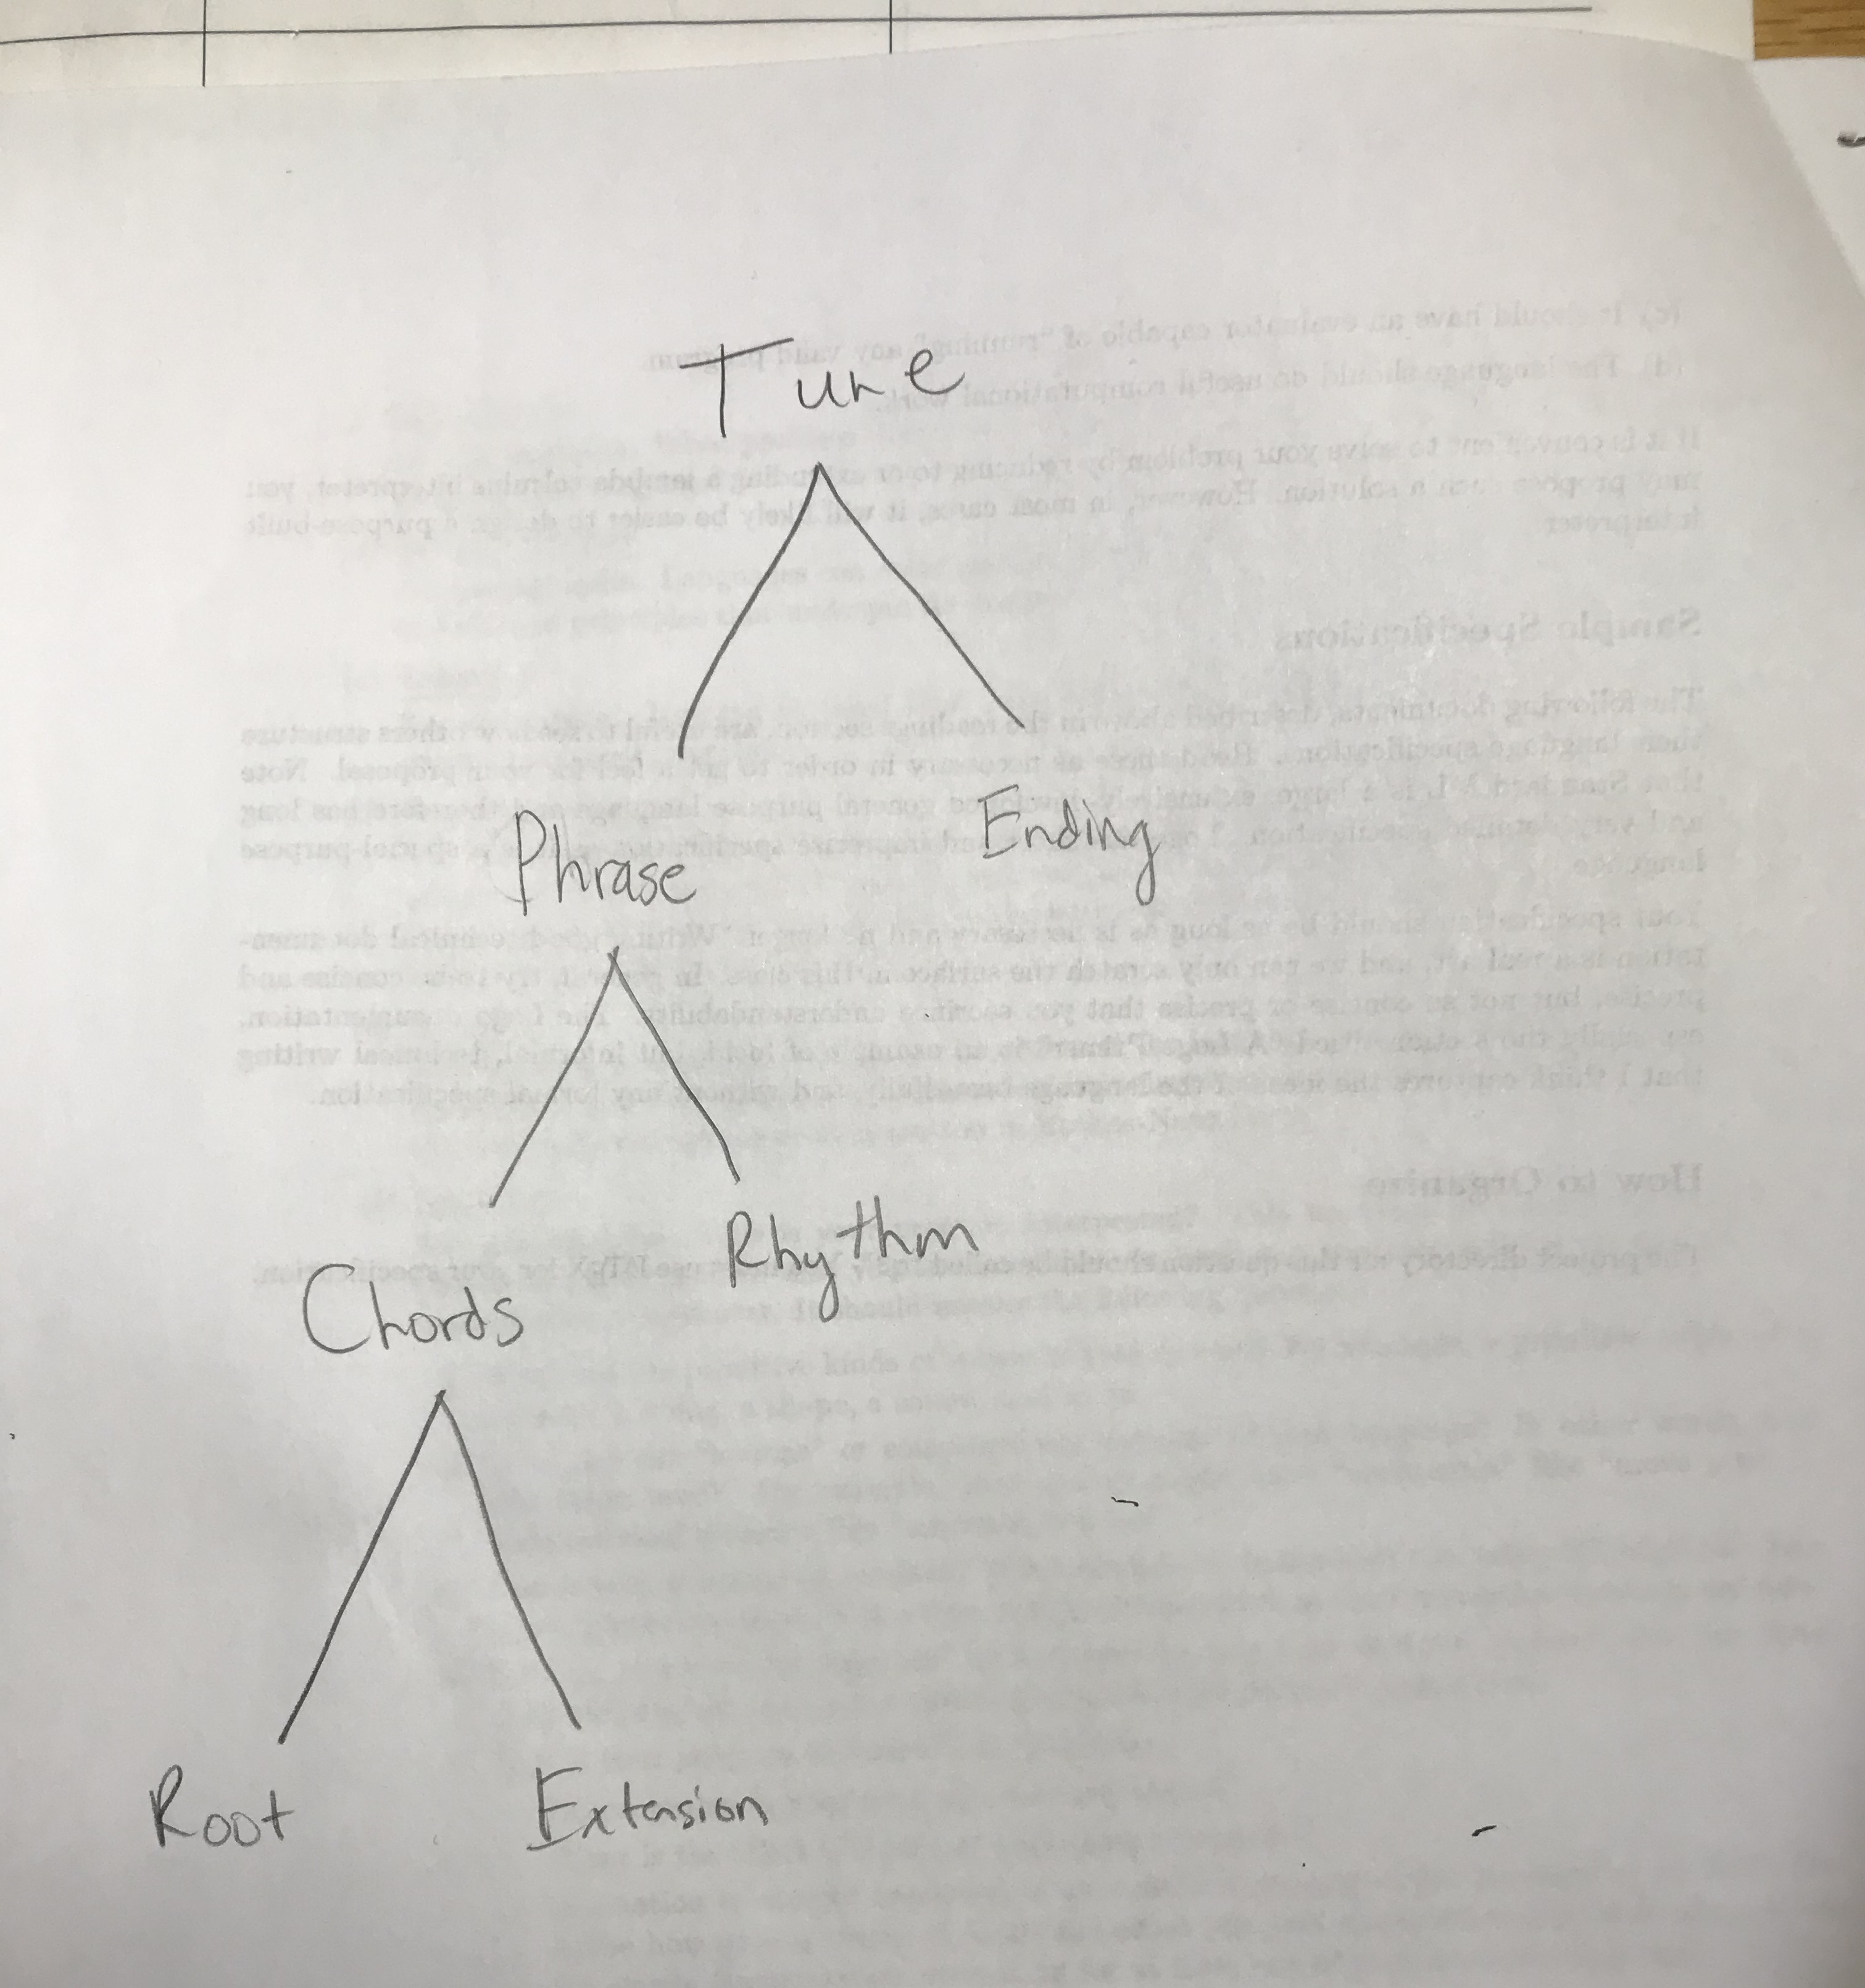
\includegraphics[scale=.09]{types.jpg}

where, roots and extensions can be further broken down into notes and symbols.

iv. Notes and symbols combine to form Roots and Extensions, which combine to form Chords. Chords and Rhythms combine to form Phrases. Phrases and Endings (or repeats) combine to form a Tune.

In example 1:
\Tree [.t [.p [.c (E,A,D,G) (-7,7,-7,7) ] (4,4,4,4) ] ending ]


\bigskip
In example 2:
\Tree [.Blues [[.A [.aChords (C,C,C,C) (7,7,7,7) ] [.rA (4,4,4,4) ] ] [.B [.bChords (C,C,F,F) (7,7,7,7) ] [.rB (4,4,4,4) ] ] [.C [.cChords (G,F,C,C) (7,7,7,7) ] [.rC (4,4,4,4) ] ]] ending ]

\bigskip
In example 3: (Only phrase A is expanded, but the same could be done for e1, e2, and B)


\Tree [.neverBeen [.A [.aChords (Bb,G,...) (ma7,-7,...) ] [.rA (2,2,...) ] ] [.e1 e1Chords re1 ] [.e2 e2Chords re2 ] [.B bChords rB ] ending ]

\bigskip
\bigskip
v. 

A. The language reads in a program as command-line input, for now, in addition to reading in the output file name. Eventually, I would like it to additionally read in info about tempo or key as well.

\bigskip
B. The effect of evaluating a program is that audio is generated. The chords entered are arpeggiated and the resulting music is written to a wav file.

\bigskip
C. A depth first, post-order traversal allows the program to store all the information about primitives to build pieces of music from the bottom up. Chords cannot be created without both a root and extensions and in turn, phrases cannot be created without the combination of chord and rhythms. As we traverse the tree, leaves and then their parents are evaluated first, allowing us to build up music from smaller pieces until we are left with complete phrases which are ultimately combined to yield a tune. (continued on next page)

Our tree for our first simple example is:
\Tree [.t [.p [.c (E,A,D,G) (-7,7,-7,7) ] (4,4,4,4) ] ending ]

If we evaluate this tree using a DFS, post-order traversal, first we evaluate the notes (E,A,D,G) and their corresponding extensions (-7,7,-7,7). Then, we combine these to form c, a list of chords. Then, combining this list of chords with a list of 4 rhythms, we have a phrase. Finally, by combining this phrase with an ending (ie. an indicator that the piece is now finished), we get t, a complete tune which is generated by the program.

\section{Remaining Work}
My next step is to implement variables and the ability to build larger, more complicated, tunes with multiple phrases. To do this, I'm planning on creating assignment operators and maintaining a dictionary of variables in my parser. Along with this, I need to clean up my parsing, and determine which types of inputs will cause programs to fail—things like negative values for rhythms or chord and rhythm lists of different lengths. Additionally, I need to figure out what I am going to do with endings—will tunes be able to be repeated, as I had originally thought or will they just automatically play once? Further, I want to add more options for playback, including different types of arpeggiation and support for different tempos and keys and more.
% DO NOT DELETE ANYTHING BELOW THIS LINE
\end{document}
